\section{The \name Approach}
\label{sec:approach}

Current parallelizing compiler designs force code analyses, transformations, and speculative techniques to work as a pipeline.
This design excludes the possibility of non-linear and fine-grain interactions between them, which makes important parallelization opportunities unreachable.
To overcome this limitation, \name introduces a compiler design where static code analyses and speculation techniques are tightly coupled to boost their discovery of parallelization opportunities (section~\ref{analyzer}).
This tight interaction generates information in the form of a dependence graph annotated with speculative assumptions.
\name's design also tightly couples code transformations with speculative assumptions to drastically reduce the overhead of the formers (section~\ref{enablers}).
These tight integrations are accomplished introducing new interfaces between compilation passes (section~\ref{enablers}) that enable their non-linear and fine-grained interactions.
These new interfaces create extra degrees of freedom, which enable \name to realize many new parallelization opportunities reaching the applicability of speculation-based approaches with the efficiency of static analyses ones.

%\name combines a speculation-aware memory analyzer, enabling
%transformations including efficient speculative privatization, and a
%parallelization planner into an exploration phase designed to find the
%best performing set of parallelization techniques.  This section
%discusses the main contributions of this paper
%(sections~\ref{analyzer},\ref{enablers},\ref{planner}), and
%presents a code example (section~\ref{motiv_example}) to underline
%improvements over Privateer~\cite{johnson:12:pldi}, a state-of-the-art
%speculative DOALL parallelization system.

%Speculative systems typically get an optimistic view of the program
%assuming application of all speculative techniques and then undo
%speculation whenever it is not needed.
%Then undo speculation whenever it was not needed.

\subsection{Planning}
%
Unlike prior speculative systems that apply a sequence of
parallelization-enabling transforms in a fixed order, \name proposes a
more sensible approach: before applying any transformation, plan
first.

Enabling transforms modify the code to remove parallelization
inhibitors, which in the context of DOALL parallelization are
cross-iteration dependences.
%
All transformations are split into two parts. The applicability guard
that participates in the planning phase of the compilation and the
actual transformation that is applied, if selected, in the
transformation phase.
%This separation of decision making and application of transformations
%allows \name to carefully select the most profitable plan.
The applicability guard utilizes memory analysis and speculative
assumptions to determine which parallelization inhibitors the
transform can handle.
%
We define speculative assumptions as predictions of program properties
based on profile information.
%
%The used speculative assumptions would need to be validated at
%runtime for the transformation to be correct.
%
The output of each applicability guard is collected in a
transformation proposal which is sent to the planner.
%
%The effect of each enabling transform is collected in a
%transformation proposal.
%
The proposal also includes a cost for the application of the
transformation itself and a set of speculative assumptions required
for the transformation to be applicable and correct.

\paragraph{Planner}

%The input to the planner is a program dependence graph and
%transformation proposals of the enabling transformations.
%
The output of the planner is the best performing set of
transformations that addresses all the parallelization inhibitors.
%
The planner is able to perform global reasoning by centralizing the
currently decentralized and greedy decision-making process found in
prior parallelizing compilers.
%
The generated plan includes a set of enabling transformations and a
set of transformations for validating speculative assumptions.
%
These are the transformations that are applied at the transformation
phase of compilation.

\subsection{Speculation-Aware Memory Analyzer}

Prior techniques use memory analysis and speculative assumptions
independently.  Instead, this work proposes a speculation-aware memory
analyzer that combines the strengths of static analysis and
cheap-to-validate speculative assumptions to reduce the need for
expensive speculation.  If memory analysis fails on its own to resolve
an analysis query, it interprets cheap-to-validate speculative
assumptions as facts ignoring the possibility of misspeculation.
%
The inclusion of speculation changes the semantics of traditional
memory analysis. It is now required to specify for each answer the
speculative assumptions, if any, that were used in the process.
%
Just applying speculation and then querying memory analysis again
would not have the same effect since the possibility of misspeculation
restrains static analysis.

\subsection{New Enabling Transformations}

%Either all static, all speculation.
Prior work on speculative parallelization often focuses on the
enabling effect of transformations without considering their cost.  To
maximize applicability, enabling transforms are often given a program
dependence structure relaxed with the use of all the available
speculative assumptions.  This approach not only creates ambiguity in
terms of what speculative assumptions are necessary but also prevents
usage of efficient variants of transformations.
%
By exposing a combination of static analysis information and
speculative assumptions, \name enables more efficient enabling
transformations.  This is especially true for the case of speculative
privatization, efficient variants of which are explored in this paper.
%
We first discuss speculative privatization as it appears in prior work
and then describe new variants that perform more efficient
privatization.

Prior software speculative systems with extended support of
privatization~\cite{johnson:12:pldi,kim:12:cgo} only infer the basic
privatization property that there are no cross-iteration data flows
for a memory object.
%
Speculative privatization application involves costly instrumentation
of all write accesses of privatized objects for logging or
communication. At commit, the private copies of each worker are merged
according to metadata that specify which worker last wrote each byte.

To avoid expensive monitoring of write sets during parallel execution
and minimize copy-out costs, we propose four efficient variants of
this transformation.
%
To be applicable, these variants require apart from the basic
privatization property additional memory object properties.

\begin{itemize}
%
\item Independent: Applicable for private objects that have no
loop-carried false dependences. This transformation's heap is shared
among all parallel workers, since there are no overlapping memory
accesses.
%
No monitoring of write sets is needed. At commit the heap is copied-out
to the non-speculative state.
%
%If the selected parallelization plan is non-speculative, then this
%heap is also shared with the main process and copy-in and copy-out
%overheads are eliminated as well.

\item Overwrite Private: Applicable for private objects that are
written at the same locations at every loop iteration (unconditionally
updated objects). This transformation's heap has CoW (copy-on-write) mapping
and at the end of the parallel invocation the last executed iteration
state is copied-out. No monitoring is needed.

%Additional applicability guard:
%object has loop-invariant condition for last update within the loop.
%
%Behavior: No write set monitoring performed. The live-out state for
%object with this property is the memory state of the last iteration
%executed before commit.

\item Predictable Private: Applicable for private objects that have
predictable live-out content. This transformation's heap has CoW mapping. The
live-out state is predictable, so no monitoring and merging parallel
workers state is needed. This transformation relies on value
prediction speculative assumptions.

\item Local Private: Applicable for private objects that are allocated
outside the loop, but all their accesses are contained within the
loop. This transformation's heap has CoW mapping and there is no copy-out
process nor monitoring.

\end{itemize}

The first two variants have been explored by Tu et
al.~\cite{ARRAY_privatization} but were limited to static analysis
based detection of privatization.  Unlike any prior work, \name
extends applicability of these variants with usage of speculative
assumptions to programs with pointers, dynamic allocation, and type
casts.







\lstset{basicstyle=\ttfamily, numbers=left, numberstyle=\tiny,
  stepnumber=1, numbersep=5pt}

\begin{figure*}[!t]
\centering
\resizebox{0.90\linewidth}{!}{
\subfloat[Privateer~\cite{johnson:12:pldi}]{
  \centering
  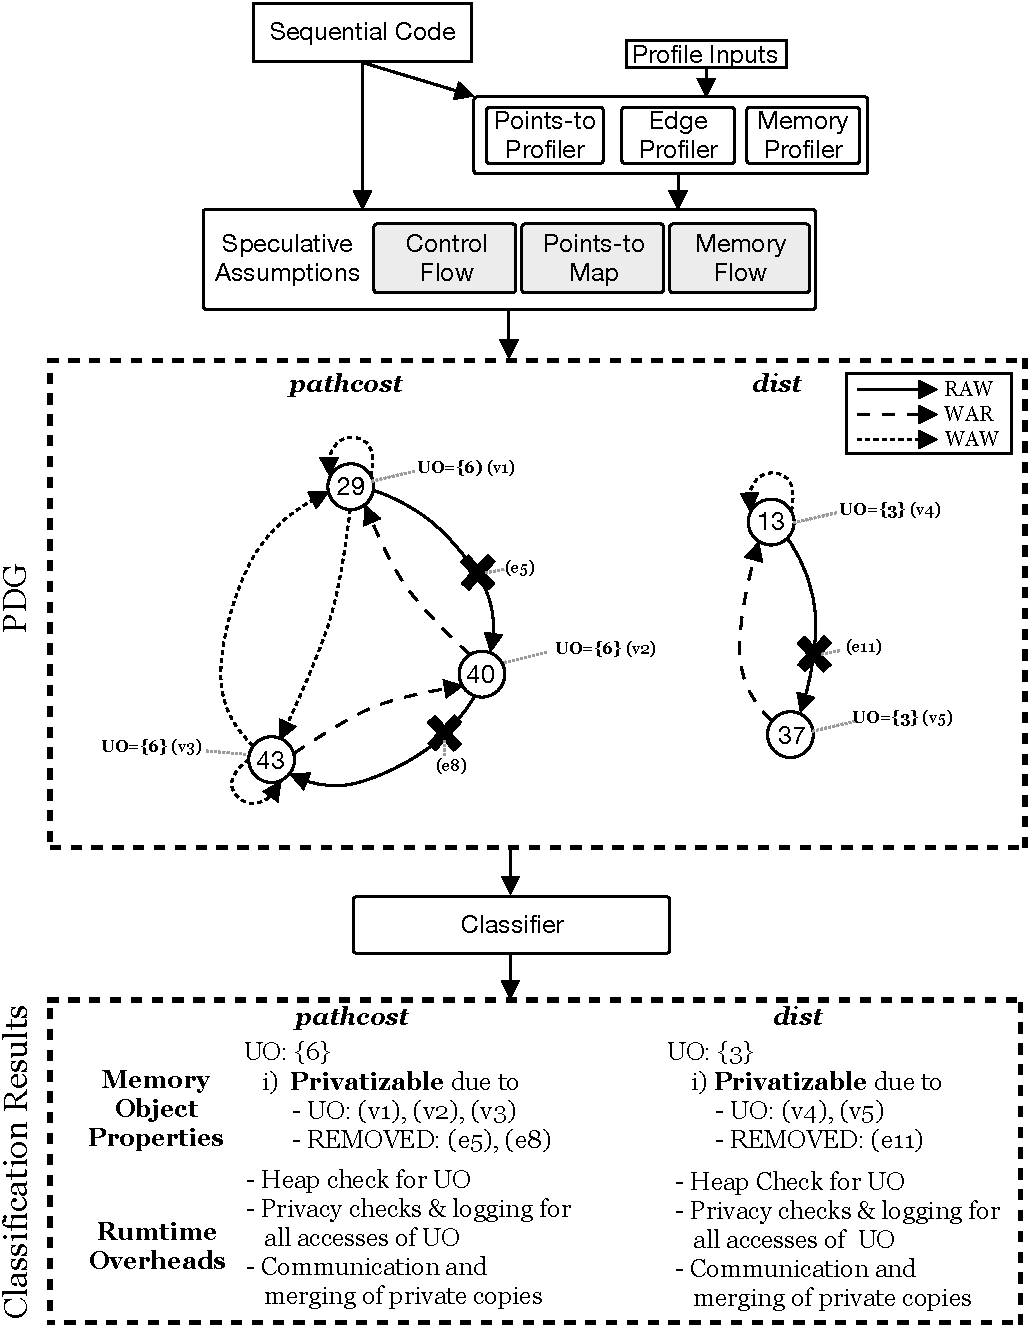
\includegraphics[width=0.46\textwidth]{figures/privateer-example-crop}
}
\qquad
\subfloat[This work]{
  \centering
  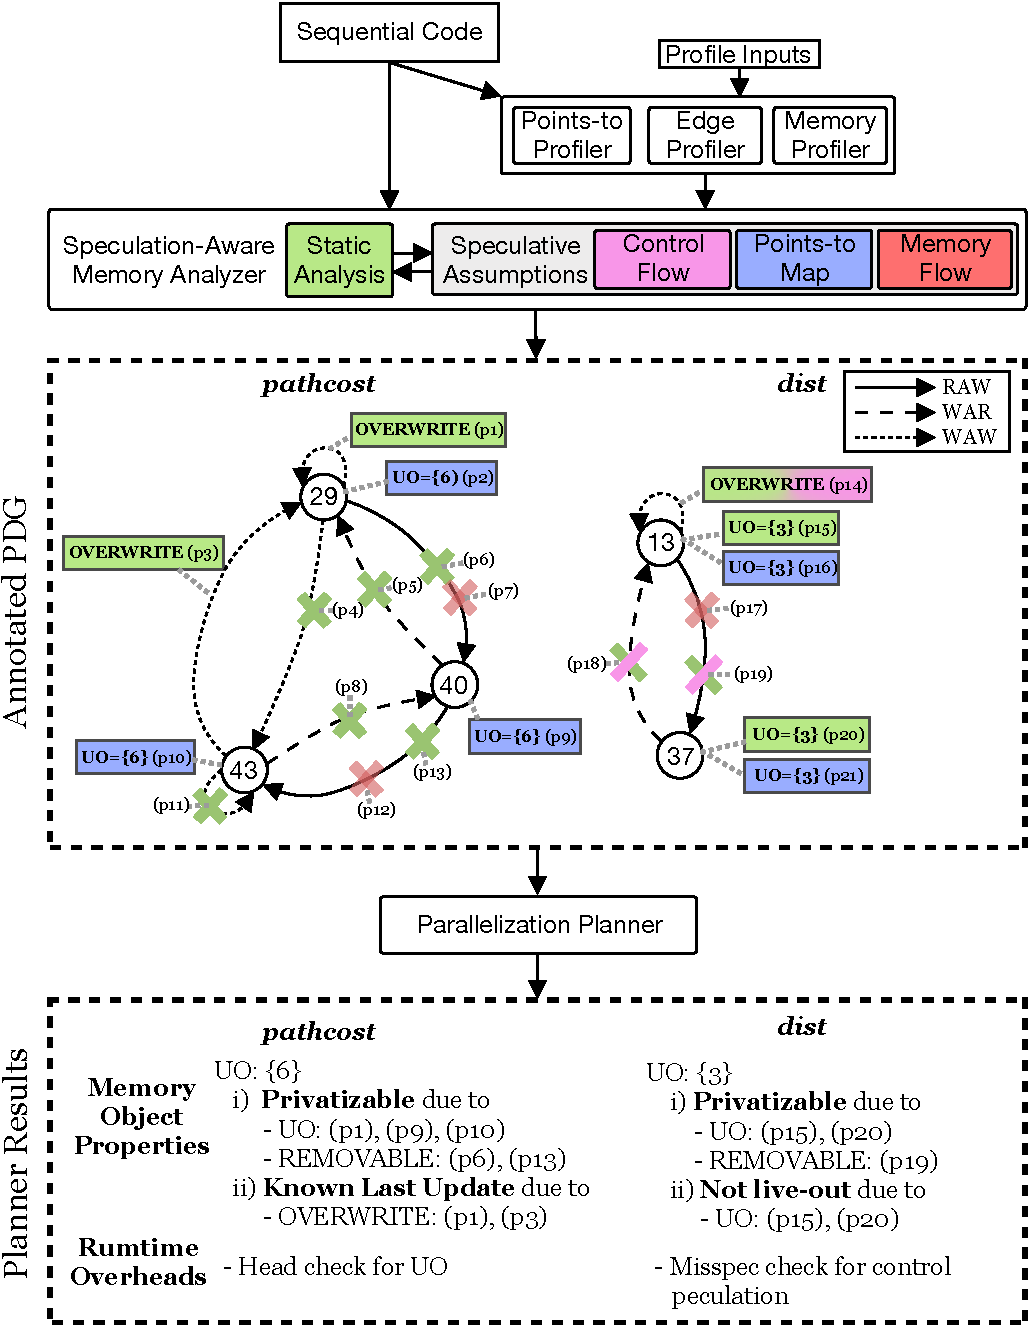
\includegraphics[width=0.46\textwidth]{figures/perspective-example-crop}
}
}
\caption{Comparison of Privateer with \name for handling memory
objects \texttt{\textbf{pathcost}} and \texttt{\textbf{dist}} of \texttt{dijkstra}}
\label{fig:dijkstra_motivation_comparison}
\end{figure*}

\begin{figure*}[!h]
\centering
\scriptsize
\resizebox{0.78\linewidth}{!}{
  % \subfloat[Sequential code]{
  %   \begin{minipage}{6cm}
  %     \begin{lstlisting}[morekeywords={pathcost,dist}, aboveskip=0pt, belowskip=0pt, firstnumber=1]
int *pathcost; // dyn alloc 1-D N
int *adj; // dyn alloc 2-D NxN
int dist;
int nDist;

void allocatePathCost() {
  pathcost = (int*)malloc(N*sizeof(int));
}

int dequeue() {
  if (!emptyQ()) {
\end{lstlisting}

\begin{lstlisting}[morekeywords={pathcost,dist}, aboveskip=0pt, belowskip=0pt,
firstnumber=13, name=dij_checks]
    dist = ...
    ...
  }
\end{lstlisting}

\begin{lstlisting}[morekeywords={pathcost,dist}, aboveskip=0pt, belowskip=0pt,
firstnumber=18, name=dij_checks]
}

void hot_loop(int N) {
\end{lstlisting}
\begin{lstlisting}[morekeywords={pathcost}, aboveskip=0pt, belowskip=0pt,
firstnumber=25]
  for (src=0; src<N; src++) {
\end{lstlisting}
\begin{lstlisting}[morekeywords={pathcost,dist}, aboveskip=0pt, belowskip=0pt,
firstnumber=28]
    for (i=0; i<N; i++)
      pathcost[i] = inf;

    enqueue(src, 0);
    while (!emptyQ()) {
      int v = dequeue();
      for (i=0; i<N; i++) {
\end{lstlisting}
\begin{lstlisting}[morekeywords={pathcost,dist}, aboveskip=0pt,
belowskip=0pt, firstnumber=38,name=dij_checks]
        nDist = adj[v][i] + dist;
\end{lstlisting}
\begin{lstlisting}[morekeywords={pathcost}, aboveskip=0pt, belowskip=0pt,
firstnumber=41]
        if (pathcost[i] > nDist) {
\end{lstlisting}
\begin{lstlisting}[morekeywords={pathcost}, aboveskip=0pt, belowskip=0pt,
firstnumber=44]
          pathcost[i] = nDist;
          enqueue(i, nDist);
        }
      }
    }
\end{lstlisting}
\begin{lstlisting}[morekeywords={pathcost}, aboveskip=0pt,
belowskip=0pt, firstnumber=52]
  }
\end{lstlisting}
\begin{lstlisting}[morekeywords={pathcost}, aboveskip=0pt,
belowskip=0pt, firstnumber=54]
}
\end{lstlisting}

  %   \end{minipage}
  %   }
\subfloat[Privateer~\cite{johnson:12:pldi}]{
  \centering
  \begin{minipage}{9.2cm}
  \begin{lstlisting}[morekeywords={pathcost}, belowskip=0pt, firstnumber=1,
name=dij_checks]
int *pathcost; // dyn alloc 1-D N
int *adj; // dyn alloc 2-D NxN
int dist, v, src, i;

for (src=0; src<N; src++) {
\end{lstlisting}

\begin{lstlisting}[morekeywords={pathcost}, aboveskip=0pt,belowskip=0pt,backgroundcolor=\color{lightgray},
firstnumber=auto, name=dij_checks]
  // Privacy Check
  private_write(pathcost, N*sizeof(int));
\end{lstlisting}

\begin{lstlisting}[morekeywords={pathcost},aboveskip=0pt, belowskip=0pt, firstnumber=auto,name=dij_checks]
  for (i=0; i<N; i++)
    pathcost[i] = inf;

  enqueue(src, 0);
  while (!emptyQ()) {
    dequeue(&v, &dist);
    for (i=0; i<N; i++) {
      nDist = adj[v][i] + dist;
\end{lstlisting}

\begin{lstlisting}[morekeywords={pathcost}, aboveskip=0pt,belowskip=0pt,backgroundcolor=\color{lightgray},
firstnumber=auto, name=dij_checks]
      // Privacy Check
      private_read(pathcost, sizeof(int));
\end{lstlisting}


\begin{lstlisting}[morekeywords={pathcost}, aboveskip=0pt, belowskip=0pt, firstnumber=auto,name=dij_checks]
      if (pathcost[i] > nDist) {
\end{lstlisting}

\begin{lstlisting}[morekeywords={pathcost}, aboveskip=0pt,belowskip=0pt,backgroundcolor=\color{lightgray},
firstnumber=auto, name=dij_checks]
        // Privacy Check
        private_write(pathcost, sizeof(int));
\end{lstlisting}

\begin{lstlisting}[morekeywords={pathcost}, aboveskip=0pt, belowskip=0pt, firstnumber=auto,name=dij_checks]
        pathcost[i] = nDist;
        enqueue(i, nDist);
      }
    }
  }
}
\end{lstlisting}

  \end{minipage}
}
\qquad
\qquad
\subfloat[This work]{
  \centering
  \begin{minipage}{7cm}
  %\begin{lstlisting}[morekeywords={pathcost}, belowskip=0pt, firstnumber=1,
%name=dij_checks]
%int *pathcost; // dyn alloc 1-D N
%int *adj; // dyn alloc 2-D NxN
%int dist, v, src, i;


\begin{lstlisting}[morekeywords={pathcost,dist}, belowskip=0pt,
firstnumber=10, name=dij_checks, showlines=true]
int dequeue() {
  if (!emptyQ()) {


\end{lstlisting}

\begin{lstlisting}[morekeywords={pathcost,dist}, aboveskip=0pt, belowskip=0pt,
firstnumber=13, name=dij_checks]
    dist = ...
    ...
  }
\end{lstlisting}

  \begin{lstlisting}[morekeywords={pathcost}, aboveskip=0pt,belowskip=0pt,backgroundcolor=\color{lightgray}, firstnumber=auto, name=dij_checks]
  else // 0% added overhead
    misspec("Control misspec in dequeue()");
\end{lstlisting}

\begin{lstlisting}[morekeywords={pathcost,dist}, aboveskip=0pt, belowskip=0pt,
firstnumber=auto, name=dij_checks,showlines=true]
}

void worker_loop(int start, int N, int step) {

\end{lstlisting}

  \begin{lstlisting}[morekeywords={pathcost}, aboveskip=0pt,belowskip=0pt,backgroundcolor=\color{lightgray},
  firstnumber=auto, name=dij_checks,showlines=true]
  // Separation Local Check -- < 0.001% added overhead
  check_heap(pathcost, OVERWRITE_PRIVATE);
  \end{lstlisting}

\begin{lstlisting}[morekeywords={pathcost}, aboveskip=0pt,
belowskip=0pt, firstnumber=24,name=dij_checks,showlines=true]

  for (src=start; src<N; src+=step) {


\end{lstlisting}
\begin{lstlisting}[morekeywords={pathcost,dist}, aboveskip=0pt,
belowskip=0pt, firstnumber=28,name=dij_checks,showlines=true]
    for (i=0; i<N; i++)
      pathcost[i] = inf;

    enqueue(src, 0);
    while (!emptyQ()) {
      int v = dequeue();
      for (i=0; i<N; i++) {
\end{lstlisting}
\begin{lstlisting}[morekeywords={pathcost,dist,nDist}, aboveskip=0pt,
belowskip=0pt, firstnumber=auto,name=dij_checks,showlines=true]



        nDist = adj[v][i] + dist;
\end{lstlisting}
\begin{lstlisting}[morekeywords={pathcost}, aboveskip=0pt,
belowskip=0pt, firstnumber=auto,name=dij_checks,showlines=true]


        if (pathcost[i] > nDist) {


\end{lstlisting}
\begin{lstlisting}[morekeywords={pathcost}, aboveskip=0pt,
belowskip=0pt, firstnumber=auto,name=dij_checks]
          pathcost[i] = nDist;
          enqueue(i, nDist);
        }
      }
    }
\end{lstlisting}

\begin{lstlisting}[morekeywords={pathcost,dist}, aboveskip=0pt,
belowskip=0pt, firstnumber=auto,name=dij_checks,showlines=true]
  }
\end{lstlisting}

\begin{lstlisting}[morekeywords={pathcost},
aboveskip=0pt,belowskip=0pt,backgroundcolor=\color{lightgray},
firstnumber=auto, name=dij_checks,showlines=true]
  // only last iter's pathcost array
  // needs to be communicated -- < 1% added overhead
  if (src == N-1+step)
    communicate_pathcost();
\end{lstlisting}

\begin{lstlisting}[morekeywords={pathcost}, aboveskip=0pt,
belowskip=0pt, firstnumber=auto,name=dij_checks]
}
\end{lstlisting}

  \end{minipage}
}
}
\caption{Parallelized code comparison of Privateer with \name for
\texttt{dijkstra}. Logging and checks during loop execution dominate the
overheads.}
\label{fig:dijkstra_motivation_comparison_source_code}
\end{figure*}
%caption,
%Checkpointing occurs every several (long running) loop iterations, thus its
%overhead is negligeable for \textit{dijkstra}.


\subsection{Example}
\label{motiv_example}

Next we describe how \name succeeds at parallelizing
\texttt{dijkstra} efficiently. This section also highlights the limitations
of prior work that blocked them as well as how the new concepts introduced
in \name overcomes them.
%
Consider again the code in Figure~\ref{fig:dijkstra_motivation},
briefly discussed~\ref{motiv_overheads}.
%
Figure~\ref{fig:dijkstra_motivation_comparison} compares the
compilation flow of \name with Privateer for handling memory objects
\texttt{\textbf{pathcost}} and \texttt{\textbf{dist}}.

\name employs an exploration phase that yields a much more profitable plan.
%The PDG is annotated by the speculation-aware memory
Notice how the PDG is annotated with properties and underlying speculative
assumptions by the speculation-aware memory analyzer. Speculation-aware
memory analyzer allows removal of the RAW dependence between instruction 13
and 37 with a combination of static analysis and control speculation. This
dependence would require usage of memory speculation in prior.
%
% Just removing dependences in the PDG creates ambiguity on how a
% dependence can be resolved, leading to over-speculation. The PDG
% contains useful properties even for non-removable dependences. For
% example,

Non-removable WAW edges in this example are annotated with
the \textit{overwrite} property that indicates that the destination
operation always overwrites the footprint of the source operation.
%
Based on the information on the PDG, three different transforms offer
handling of memory objects, and \textbf{overwrite privatization} and
\textbf{local privatization} are new enablers proposed in
section~\ref{enablers}.

%For example, handling of \textit{dist} requires usage of control
%speculation (for the branch in line 11,
%fig.~\ref{fig:dijkstra_motivation}).
%
%Notice that \textit{dist} can be handled by all three
%transformations.
%
The DOALL planner then selects the lowest cost solution for each memory
object. For example, for \texttt{\textbf{dist}} the local privatization's
offer is selected since it is the cheapest privatization transform and its
speculative assumption is the same as other options'.
\texttt{\textbf{nDist}} object (not shown in this figure) is also handled
by local privatization. \texttt{\textbf{pathcost}} is resolved by overwrite
privatization.
% %
% Extracting this efficient plan would not be possible without the use
% speculation-aware memory analyzer and efficient speculative
% privatization transformations.

% From prior work, Privateer~\cite{johnson:12:pldi} is the only
% automatic system to support privatization of dynamically allocated
% objects, like \textit{pathcost}, even in the presence of unrestricted
% pointers.


%
Privateer, on the other hand, without the support of speculation-aware
memory analyzer and  efficient speculative privatization transform, relies
on profile information to infer that these two objects are privatizable and
is forced to apply transforms with privacy checks and merging of private
copies, resulting in high runtime overheads.

%Even if memory analysis was used instead of memory speculation, the
%classifier sees the optimistic view of the program
%


%not only in Privateer but in any other automatic parallelization
%speculative system.


%Whilst the private property is enough for DOALL
%Notice that we infer an additional property that improves the profitability
%of parallelization.

%For inferring the property that a private memory object has the additional local-private
%property, it suffices to identify all accesses of the memory object
%and check that all of them are within the loop.
%locally-accessed property.


Figure~\ref{fig:dijkstra_motivation_comparison_source_code} compares the
resulting parallelized versions (in a simplified form) for \name and
Privateer. The code includes all the added checks, logging and handling
live-out overheads. The code changes are marked with the average added
overhead over the useful work of each worker. It is clear that \name is
able to parallelize \texttt{dijkstra} with minimum overheads thanks to the
use of speculative-aware memory analyzer, careful selection of applied
transformations, and use of efficient privatization variants. In fact,
\name exhibits 4.8$\times$ speedup over Privateer for \texttt{dijkstra}
(see~\ref{eval}).

%Privateer would choose to just do simple privatization with mem spec.
%The spec-aware analyzer allows removal of mem spec and efficient
%privatization in this case.
%
%\begin{itemize}
%\item
%Privatization of these memory objects requires:
%\begin{enumerate}
%\item
%identification of all accesses of these objects
%    within the loop
%\item
%absence of cross-iteration flow
%     dependences on each of these accesses
%\end{enumerate}
%
%\end{itemize}
%
%
%DOALL can become applicable if these two objects are proven to have the
%private property.
%
%We compare our approach where we combine static analysis with cheap-to-validate
%with privateer's monolithic approach that over-speculates and is limited by high
%runtime overheads.
%
%Note that anti-dependences are ignored since both systems use
%process-based runtime systems.
